\documentclass[12pt]{article}
\usepackage{amsmath, amssymb}
\usepackage{graphicx}
\usepackage{fancyhdr}
\usepackage{enumitem}
\usepackage{multicol}
\usepackage{geometry}
\usepackage{listings}
\usepackage{tikz}
\usepackage{xcolor}
\geometry{margin=1in}

% Header
\pagestyle{fancy}
\fancyhf{}
\rhead{Devi Rosa Aprilla}
\lhead{Assignment}
\cfoot{\thepage}

% TikZ & Listings configurations (font lebih kecil)
\usetikzlibrary{arrows.meta, positioning}
\definecolor{javared}{rgb}{0.6,0,0}
\definecolor{javagreen}{rgb}{0.25,0.5,0.35}
\definecolor{javapurple}{rgb}{0.5,0,0.35}
\definecolor{javacommentblue}{rgb}{0.25,0.35,0.75}
\lstset{
language=Java,
basicstyle=\ttfamily\scriptsize, % font lebih kecil
keywordstyle=\color{javapurple}\bfseries,
stringstyle=\color{javared},
commentstyle=\color{javacommentblue},
morecomment=[s][\color{javacommentblue}]{/**}{*/},
numbers=left,
numberstyle=\tiny\color{black},
stepnumber=1,
numbersep=8pt,
showspaces=false,
showstringspaces=false,
tabsize=2,
breaklines=true,
frame=single,
frameround=tttt,
captionpos=b
}
\tikzset{
    umlclass/.style={
        rectangle,
        draw=black,
        text width=6cm,
        minimum height=0.7cm,
        text ragged,  
        font=\scriptsize % font lebih kecil
    },
    umltitle/.style={
        rectangle,
        draw=black,
        text width=6cm,
        minimum height=0.7cm,
        text centered, 
        font=\bfseries\scriptsize, % font lebih kecil
        fill=gray!20
    },
    inheritance/.style={-{Triangle[length=2mm, width=2mm]}, line width=1pt}
}

\begin{document}

\begin{center}
    {Evaluasi Akhir Semester 2025}\\
    \textit{Algoritma dan Pemrograman Komputer 2}\\
\end{center}

\vspace{0.1cm}

\begin{enumerate}
    \item Perhatikan listing program berikut. Jawaban pertanyaan yang diberikan.
    
    \begin{lstlisting}
package eas_no_1;
public class EAS_no_1 {
    public static void main(String[] args) {
        Car chevy = new Car( );
        MotorCycle harley = new MotorCycle( 3 );
        MotorCycle honda = new MotorCycle( );
        System.out.println( chevy.toString( ) );
        System.out.println( harley.toString( ) );
        System.out.println( honda.toString( ) );
    }
}
// Vehicle class
class Vehicle {
    private int nrWheels;
    
    public Vehicle( )
    { this( 4 ); }
    public Vehicle ( int nrWheels )
    { setWheels( nrWheels); }
    public String toString( )
    { return "Vehicle with " + getWheels() + " Wheels";}
    public int getWheels( )
    { return nrWheels; }
    public void setWheels ( int wheels )
    { nrWheels = wheels; }
}

// MotorCycle class
class MotorCycle extends Vehicle {
    public MotorCycle( )
    { this( 2 ); }
    public MotorCycle( int wheels )
    { super( wheels ); }
}

// Car class
class Car extends Vehicle
{
    public Car( )
    { super( 4 ); }
    public String toString( )
    {
        return "Car with " + getWheels() + " wheels";
    }
}
    \end{lstlisting}

    \begin{enumerate}[label=\alph*)]
        \item Terangkan langkah demi langkah sehingga menghasilkan keluaran yang benar.
        \item Jika objek Car dibuat, jelaskan urutan konstruktor-konstruktor yang dipanggil.
        \item Pada konstruktor Vehicle, apa maksud dari pernyataan \texttt{\{ this( 4 ); \}}
        \item Pada konstruktor MotorCycle, apa maksud dari pernyataan \texttt{\{ super(wheels); \}?}
        \item Method \texttt{toString()} pada class Car invokes \texttt{getWheels()}, meskipun \texttt{getWheels()} tidak terdefinisi pada class Car. Bagaimana ini terjadi?
    \end{enumerate}

    \vspace{0.5cm}

    \item Desain kelas bernama TitikQu untuk mewakili titik dengan koordinat x dan y. Kelas berisi:

    \begin{itemize}
        \item[$\checkmark$] Data x dan y yang mewakili koordinat
        \item[$\checkmark$] Lengkapi dengan metode GetData dan setData
        \item[$\checkmark$] Konstruktor no-arg yang menciptakan titik (0, 0).
        \item[$\checkmark$] Konstruktor yang membangun titik dengan koordinat tertentu.
        \item[$\checkmark$] Metode bernama \texttt{jarak()} tanpa argument yang mengembalikan nilai jarak dari objek titik ini ke titik pusat(0,0).
        \item[$\checkmark$] Metode bernama \texttt{Gradient(TitikQu T)} dengan argument titik yang mengembalikan nilai gradient (double) dari garis yang melalui dua titik
    \end{itemize}

    Tulis program pengujian yang menciptakan dua titik (3,8) dan (10, 30.5) dan menampilkan jarak titik tersebut dengan titik pusat. Juga menampilkan gradient yang terbentuk dari dua titik tersebut.

    \vspace{0.5cm}

    \item Perhatikan listing program berikut:

    \begin{enumerate}[label=\alph*.]
        \item Temukan error dari program berikut dan perbaiki
        \item Apa yang dikerjakan oleh program setelah perbaikan (jelaskan tahap-demi-tahap) sehingga menghasilkan keluaran yang benar.
    \end{enumerate}

    (HINT: dynamic binding)

    \begin{lstlisting}
package EAS2025;

public class soalEAS_No3 {

    public static void main(String[] args) {
        Parent a = new subclass1();
        a.Print();
        a.Haloo();
        
        Parent b = new subclass2();
        b.Print();
        b.Cetak();
    }
}

class Parent {
    void Print() {
        System.out.println("parent class");
    }
    
    void Haloo() {
        System.out.println("Haloo JAVA");
    }
}

class subclass1 extends Parent {
    void Print() {
        System.out.println("subclass1");
    }
}

class subclass2 extends Parent {
    void Print() {
        System.out.println("Print : subclass2");
    }
    
    void Cetak(){
        System.out.println("Cetak : subclass2");
    }
}
    \end{lstlisting}

    \vspace{0.5cm}

    \item Perhatikan DENGAN SEKSAMA DAN TELITI Diagram UML berikut:

    \begin{center}
    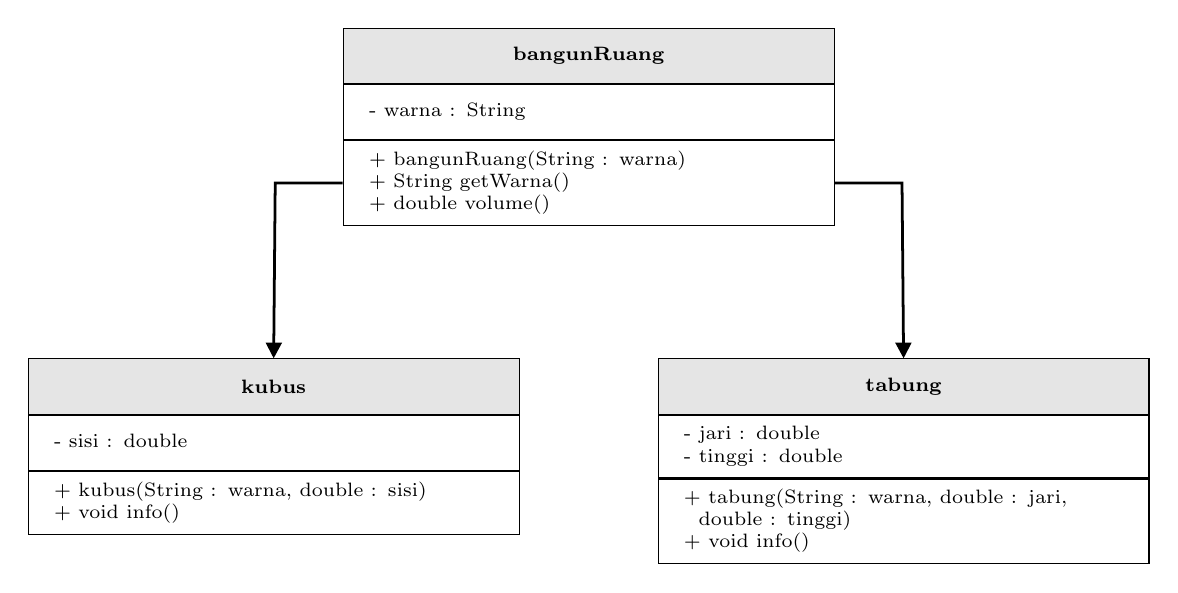
\begin{tikzpicture}

    \tikzset{
        umlclass/.style={
            rectangle,
            draw=black,
            text width=6cm,
            minimum height=0.7cm,
            text ragged,  
            font=\scriptsize
        },
        umltitle/.style={
            rectangle,
            draw=black,
            text width=6cm,
            minimum height=0.7cm,
            text centered, 
            font=\bfseries\scriptsize,
            fill=gray!20
        },
        inheritance/.style={-{Triangle[length=2mm, width=2mm]}, line width=1pt}
    }

    \node[umltitle] (super) at (-2,0) {bangunRuang};
    \node[umlclass, anchor=north west] (superattr) at ([xshift=0cm]super.south west) {
    \begin{tabular}{l}
    - warna : String
    \end{tabular}
    };
    \node[umlclass, anchor=north west] (supermeth) at ([xshift=0cm]superattr.south west) {
    \begin{tabular}{l}
    + bangunRuang(String : warna)\\
    + String getWarna()\\
    + double volume()
    \end{tabular}
    };

    \node[umltitle] (kubus) at (-6,-4.2) {kubus};
    \node[umlclass, anchor=north west] (kubusattr) at ([xshift=0cm]kubus.south west) {
    \begin{tabular}{l}
    - sisi : double
    \end{tabular}
    };
    \node[umlclass, anchor=north west] (kubusmeth) at ([xshift=0cm]kubusattr.south west) {
    \begin{tabular}{l}
    + kubus(String : warna, double : sisi)\\
    + void info()
    \end{tabular}
    };

    \node[umltitle] (tabung) at (2,-4.2) {tabung};
    \node[umlclass, anchor=north west] (tabungattr) at ([xshift=0cm]tabung.south west) {
    \begin{tabular}{l}
    - jari : double\\
    - tinggi : double
    \end{tabular}
    };
    \node[umlclass, anchor=north west] (tabungmeth) at ([xshift=0cm]tabungattr.south west) {
    \begin{tabular}{l}
    + tabung(String : warna, double : jari,\\
    \ \ double : tinggi)\\
    + void info()
    \end{tabular}
    };

    \draw[inheritance]
        (supermeth.west) -- ++(-0.856,0) -- (kubus.north);

    \draw[inheritance]
        (supermeth.east) -- ++(0.856,0) -- (tabung.north);

    \end{tikzpicture}
    \end{center}

    Keterangan: Method Info di kelas kubus dan tabung akan mencetak warna dan volume

    \begin{enumerate}[label=\alph*)]
        \item Implementasikan diagram kelas pada UML diatas dalam sebuah kode program
        \item Buat kelas main untuk menguji/menjalankan program yang anda buat tersebut
    \end{enumerate}

\end{enumerate}

\vspace{1cm}
\begin{center}
    \textasciitilde\ Selamat Mengerjakan\textasciitilde
\end{center}

\end{document}